\documentclass[10pt]{beamer}
\usepackage[T1]{fontenc}
\usepackage[utf8]{inputenc}

\usepackage{graphicx}
\usepackage{booktabs}
\usepackage{multirow}

\usepackage{amssymb,amsmath,amsthm,amsfonts,mathtools}

\usepackage[autostyle,italian=guillemets]{csquotes}
\usepackage[backend=biber]{biblatex}
\addbibresource{../theory-of-truss-structures/bib.bib}

\usepackage{pgfplots}
\usetikzlibrary{calc}
\usetikzlibrary{patterns}
\usetikzlibrary{hobby}

\usetheme{default}
\useinnertheme{circles}
\useoutertheme{infolines}

\definecolor{padova}{RGB}{155,0,20}
\definecolor{padova-nero}{RGB}{72,79.,89}
\definecolor{grigio}{gray}{0.97}
\setbeamercolor{palette primary}{fg=white,bg=padova}
\setbeamercolor{palette secondary}{fg=white,bg=padova}
\setbeamercolor{palette tertiary}{fg=white,bg=padova}
\setbeamercolor{titlelike}{fg=white,bg=padova-nero}
\setbeamercolor{title}{fg=black,bg=white}
\setbeamercolor{normal text}{fg=black,bg=white}
\setbeamercolor{block body}{fg=black,bg=white}
\setbeamercolor{block title}{fg=black,bg=white}
\setbeamercolor{alerted text}{fg=black,bg=white}
\setbeamercolor{local structure}{fg=padova,bg=white}

\setbeamerfont{block title}{series=\bfseries,size=\normalsize}
\setbeamerfont{alerted text}{series=\bfseries,size=\normalsize}


\setbeamertemplate{navigation symbols}{}

\title[]{Numerical solution of the statics problem for nonlinear elastic truss structures}
\author[]{Bernardo Ardini}
\date{Padova, 16 dicembre 2024}

\theoremstyle{definition}
\newtheorem{proposizione}{Proposition}
\newtheorem{definizione}{Definition}
\newtheorem{teorema}{Theorem}
\newtheorem{corollario}{Corollario}
\newtheorem{mylemma}[proposizione]{Lemma}
\newtheorem*{nota}{Nota}
\newtheorem*{esempio}{Esempio}

\DeclareMathOperator{\cof}{cof}
\DeclareMathOperator{\diver}{div}
\DeclareMathOperator{\vol}{vol}
\DeclareMathOperator{\are}{area}
\DeclareMathOperator{\supp}{supp}
\DeclareMathOperator{\diag}{diag}
\DeclareMathOperator{\so}{SO}
\DeclareMathOperator{\tr}{tr}

\DeclarePairedDelimiter{\norma}{\lVert}{\rVert}
\DeclarePairedDelimiter{\funz}{\langle}{\rangle}

\newcommand{\dind}[2]{\frac{\partial #1}{\partial #2}}

\newcommand{\omissis}{[\textellipsis\unkern]}
\newcommand{\x}{x}
\newcommand{\y}{u}
\newcommand{\z}{y}
\newcommand{\A}{\mathfrak{A}}
\newcommand{\lin}{\text{Mat}}
\newcommand{\sotre}{\text{Orth}^+}
\newcommand{\orth}{\text{Orth}}
\newcommand{\sym}{\text{Sym}}

\newcommand{\rie}{\hspace{3cm}}
\newcommand{\tol}{\text{tol}}

\begin{document}

\begin{frame}
\maketitle
\end{frame}

\begin{frame}
\frametitle{The truss structure}

\begin{columns}
\begin{column}{0.4\framewidth}
\begin{block}{Vertices}
$U=\{1,\dots,n\}$, vertex $v\in U$ occupies a position $x^{(v)}\in\mathbb{R}^3$
\end{block}
\end{column}
\begin{column}{0.5\framewidth}
\begin{block}{Elements}
$\mathcal{E}\subset\{(v,w)\;|\;\text{$v,w\in U$ and $v<w$}\}$ \\
element $(v,w)$ connect $v$ with $w$
\end{block}
\end{column}
\end{columns}

\begin{columns}
\begin{column}{0.6\framewidth}
\begin{block}{Example}
Vertices $U=\{1,2,3,4\}$ \\
Elements $\mathcal{E}=\{(1,2),(2,3),(3,4),(1,3)\}$
\end{block}
\end{column}
\begin{column}{0.3\framewidth}
\begin{center}
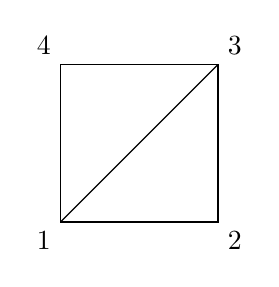
\begin{tikzpicture}[scale=2]
\draw (0,0) -- (0,1) -- (1,1) -- (1,0) -- cycle;
\draw (0,0) -- (1,1);
\node[anchor=north east] at (0,0) {1};
\node[anchor=north west] at (1,0) {2};
\node[anchor=south west] at (1,1) {3};
\node[anchor=south east] at (0,1) {4};
\end{tikzpicture}
\end{center}
\end{column}
\end{columns}

\begin{block}{Configuration and reference configuration}
\begin{itemize}
\item Configuration fully described by $\{x^{(v)}\}_{v\in U}$
\item We call $\{X^{(v)}\}_{v\in U}$ the reference configuration of the structure
\end{itemize}
\end{block}

\end{frame}

\begin{frame}
\frametitle{Tensions and constitutive relations}

\begin{columns}
\begin{column}{0.4\framewidth}
Fixed a configuration $\{x^{(v)}\}_{v\in U}$ \\
\begin{block}{Element tension}
To each element $(v,w)\in\mathcal{E}$ we assign a tension $T^{(v,w)}$
\end{block}
\begin{block}{Constitutive relation}
Describe the particular behavior of the material
\[
T^{(v,w)}=\hat{T}^{(v,w)}(x^{(w)}-x^{(v)})
\]
\end{block}
\end{column}
\begin{column}{0.5\framewidth}
\begin{block}{Example}
We will use
\[
\hat{T}(\Delta x)=EV\epsilon\frac{\Delta x}{|\Delta x|^2}
\]
where
\begin{itemize}
\item $V$ referential volume of element
\item  $E$ Young modulus
\item $\epsilon=\log\frac{|\Delta x|}{L}$ logarithmic strain
\item $L$ referential length of element
\end{itemize}
\end{block}
\end{column}
\end{columns}

\end{frame}

\begin{frame}
\frametitle{Tensions and constitutive relations}

\begin{columns}
\begin{column}{0.6\framewidth}
\begin{block}{Vertex tension}
For each vertex $v\in U$ we define
\[
T^{(v)}=\sum_{e\in\mathcal{E}}s(e,v)T^{(e)}
\]
where $s(e,v)\in\{0,\pm1\}$ take into account whether $v$ is $e_1$ or $e_2$ with $e=(e_1,e_2)$
\[
s(e,v)=
\begin{cases}
1 & \text{if $v=e_1$} \\
-1 & \text{if $v=e_2$} \\
0 & \text{otherwise} \\
\end{cases}
\]
\end{block}
\end{column}
\begin{column}{0.4\framewidth}
\begin{center}
\begin{tikzpicture}[scale=1.3,>=latex]
\draw (0,0) -- ++(10:1);
\draw (0,0) -- ++(130:1);
\draw (0,0) -- ++(250:1);
\draw[->] (10:1) -- (10:0.5);
\draw[->] (0,0) -- (130:0.5);
\draw[->] (0,0) -- (250:0.5);
\draw [fill=black] (0,0) circle (0.05);
\node[anchor=east] at (0,0) {2};
\node[anchor=west] at (10:1) {1};
\node[anchor=south east] at (130:1) {3};
\node[anchor=north] at (250:1) {4};
\end{tikzpicture}
\end{center}
\end{column}
\end{columns}

\end{frame}

\begin{frame}

\frametitle{The statics problem}

\begin{block}{Some definitions}
\begin{itemize}
\item $W=\{1,\dots,m\}\subset U$ mobile vertices
\item $V=U\setminus W$ fixed vertices
\item $\{X^{(v)}\}_{v\in U}$ reference configuration
\item $X=\{X^{(w)}\}_{w\in W}\in\mathbb{R}^{3m}$ reference positions of mobile vertices
\item $x=\{x^{(w)}\}_{w\in W}\in\mathbb{R}^{3m}$ positions of mobile vertices
\item $T=T(x)=\{T^{(w)}\}_{w\in W}\in\mathbb{R}^{3m}$ tensions on mobile vertices
\item $F=\{F^{(w)}\}_{w\in W}\in\mathbb{R}^{3m}$ external forces on mobile vertices
\end{itemize}
\end{block}

\begin{block}{Problem}
To find $x\in\mathbb{R}^{3m}$ such that
\[
T(x)+F=0
\]
\end{block}

\end{frame}

\begin{frame}

\frametitle{The statics problem}

\begin{columns}
\begin{column}{0.7\framewidth}
\begin{block}{Stiffness matrix}
Defined as the Jacobian matrix $K(x)=DT(x)$ \\
It tell us how much the structure if stiff at configuration $x$
\end{block}
\begin{teorema}[local existence and uniqueness result]
Let $T\in C^1(\Omega)$ with $\Omega\subset\mathbb{R}^{3m}$ open. Let $x_0\in\mathbb{R}^{3m}$ and $F_0\in\mathbb{R}^{3m}$ be such that
\begin{enumerate}
\item $\det DT(x_0)\neq0$,
\item $T(x_0)+F_0=0$.
\end{enumerate}
Then there exists $\delta>0$ and $\epsilon>0$ such that for every $F\in B(F_0,\delta)$ there exists a unique $x\in\mathbb{R}^{3m}$ solution of $T(x)+F=0$.
\end{teorema}
\begin{proof}
Simple application of Inverse Function Theorem
\end{proof}
\end{column}
\begin{column}{0.3\framewidth}
\begin{center}
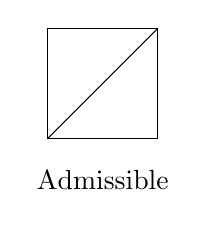
\begin{tikzpicture}[scale=1.4]
\draw (0,0) -- (0,1) -- (1,1) -- (1,0) -- cycle;
\draw (0,0) -- (1,1);
\node[anchor=north] at (0.5,-0.2) {Admissible};
\end{tikzpicture}
\end{center}
\vspace{20pt}
\begin{center}

\begin{tikzpicture}[scale=1.4]
\draw (0,0) -- (0,1) -- (1,1) -- (1,0) -- cycle;
\node[anchor=north] at (0.5,-0.2) {Not admissible};
\end{tikzpicture}
\end{center}
\end{column}
\end{columns}

\end{frame}

\begin{frame}

\frametitle{Newton-Raphson method}

\begin{columns}
\begin{column}{0.5\framewidth}
\begin{block}{Idea}
We want to find the equilibrium configuration of the structure given an external load $F$
\begin{enumerate}
\item<1-> Start in reference configuration with zero tensions and $F_0=0$ external forces
\item<2-> Increment the external load of $\delta F=\frac{F}{N}$ and find the local solution via Newton method
\item<3-> repeat previous step until $F$ is reached
\end{enumerate}
\end{block}
\end{column}
\begin{column}{0.5\framewidth}
\begin{center}
\end{center}
\includegraphics<1>[width=0.4\framewidth]{immagini/arch1.pdf}%
\includegraphics<2>[width=0.4\framewidth]{immagini/arch3.pdf}%
\includegraphics<3>[width=0.4\framewidth]{immagini/arch8.pdf}%
\includegraphics<4>[width=0.4\framewidth]{immagini/arch11.pdf}%
\includegraphics<5>[width=0.4\framewidth]{immagini/arch15.pdf}%
\end{column}
\end{columns}

\end{frame}

\begin{frame}

\frametitle{Newton-Raphson method}

\begin{columns}
\begin{column}{0.45\textwidth}
\begin{onlyenv}<1>
\begin{block}{Newton method}
If we want so solve
\[
T(x+\delta x)+F=0,
\]
we make the linearization
\[
\begin{split}
T(x+&\delta x)+F\simeq R+K(x)\delta x.
\end{split}
\]
and then
\[
\delta x=-K^{-1}R.
\]
Repeat until tolerance is reached
\end{block}
\end{onlyenv}
\begin{onlyenv}<2>
\begin{block}{Solving the linear system}
To compute $\delta x=-K^{-1}R$ we perform LU factorization
\begin{enumerate}
\item compute $L$ and $U$ such that $K=LU$
\item compute $y=L^{-1}R$ by forward substitution
\item compute $\delta x=-U^{-1}y$ by backward substitution
\end{enumerate}
\end{block}
\end{onlyenv}
\begin{onlyenv}<3>
\begin{block}{What we can make parallel?}
\begin{itemize}
\item computation of $T(x)$ and $K(x)$
\item LU factorization
\end{itemize}
\end{block}
\end{onlyenv}
\end{column}
\begin{column}{0.5\framewidth}
\begin{block}{Algorithm}
Input: $\{X^{(v)}\}_{v\in U}$, $\{F_j\}_{j=0,\dots,N}$
\begin{itemize}
\item $x=X$
\item For $j$ from $1$ to $N$ do\\
\begin{itemize}
\item $F=F_j$
\item $T=T(x)$
\item $K=K(x)$
\item $R=T(x)+F$
\item While $\frac{R}{F}>\tol$
\begin{enumerate}
\item $\delta x=-K^{-1}R$
\item $x=x+\delta x$
\item $T=T(x)$
\item $K=K(x)$
\item $R=T(x)+F$
\end{enumerate}
\item End do
\end{itemize}
\item End do
\end{itemize}
\end{block}
\end{column}
\end{columns}

\end{frame}

\begin{frame}
\frametitle{Computation of $T(x)$ and $K(x)$}

\begin{columns}
\begin{column}{0.35\textwidth}
We consider only $T(x)$ for simplicity
\begin{block}{Irregular parallelism}
\begin{itemize}
\item we parallelize the external loop
\item when $s(e,w)=0$ we do not need to compute anything
\item we use tasks
\end{itemize}
\end{block}
\end{column}
\begin{column}{0.5\framewidth}
\begin{block}{Algorithm}
Input: $x$, $X$ \\
$T=0$ \\
For $w\in W$ do\\
\begin{itemize}
\item[] For $e\in\mathcal{E}$ do
\begin{itemize}
\item[] If $s(e,w)\neq 0$ do
\begin{itemize}
\item[] $T^{(e)}=\hat{T}^{(e)}(x^{(e_2)}-x^{(e_1)})$
\item[] $T^{(w)}=T^{(w)}+s(e,w)$
\end{itemize}
\item[] End do
\end{itemize}
\item[] End do
\end{itemize}
End do
\end{block}
\end{column}
\end{columns}

\end{frame}

\begin{frame}
\frametitle{LU factorization}

\begin{onlyenv}<1>
\begin{columns}
\begin{column}{0.4\framewidth}
\begin{block}{Problem}
Given suitable $A\in\mathbb{R}^{n\otimes n}$ we have to compute $L$ and $U$ such that $A=LU$
\end{block}
\end{column}
\begin{column}{0.4\framewidth}
\begin{block}{Idea}
We decompose each matrix in four blocks with $A_{11}\in\mathbb{R}^{m\otimes m}$ where $m<n$ (e.g. $n=600$ and $m=70$)
\end{block}
\end{column}
\end{columns}

\begin{columns}
\begin{column}{0.3\framewidth}
\[
A=\left(
\begin{array}{c|c}
A_{11} & A_{12} \\
\hline
A_{21} & A_{22}
\end{array}
\right)
\]
\end{column}
\begin{column}{0.3\framewidth}
\[
L=\left(
\begin{array}{c|c}
L_{11} & 0 \\
\hline
L_{21} & L_{22}
\end{array}
\right)
\]
\end{column}
\begin{column}{0.3\framewidth}
\[
U=\left(
\begin{array}{c|c}
U_{11} & U_{12} \\
\hline
0 & U_{22}
\end{array}
\right)
\]
\end{column}
\end{columns}
\end{onlyenv}

\begin{columns}
\begin{column}{0.4\framewidth}
\begin{block}{New problem}
To find $L_{ij}$ and $U_{ij}$ such that
\begin{enumerate}
\item $A_{11}=L_{11}U_{11}$
\item $A_{12}=L_{11}U_{12}$
\item $A_{21}=L_{21}U_{11}$
\item $A_{22}=L_{22}U_{22}$
\end{enumerate}
\end{block}
\end{column}
\begin{column}{0.5\framewidth}
\begin{block}{Solution}
\begin{enumerate}
\item find $L_{11}$ and $U_{11}$ with serial algorithm (Gauss elimination)
\item find $U_{12}$ with forward substitution
\item find $L_{21}$ with backward substitution
\item find $L_{22}$ and $U_{22}$ recursively
\end{enumerate}
\end{block}
\end{column}
\end{columns}

\begin{onlyenv}<3>
\begin{columns}

\begin{column}{0.3\framewidth}
\begin{block}{Parallelization}
Both step (2) and (3) can be performed in parallel
\end{block}
\end{column}

\begin{column}{0.65\framewidth}
\begin{block}{For example for step (2)}
If we want to find $U_{12}$ from $A_{12}=L_{11}U_{12}$ we write $U_{12}=(b_1|\dots|b_{n-m})$ and $A_{12}=(a_1|\dots|a_{n-m})$ and we solve in parallel $b_i=L_{11}^{-1}a_i$ 
\end{block}
\end{column}
\end{columns}
\end{onlyenv}

\end{frame}

\begin{frame}
\frametitle{Speedup}

\begin{center}
\begin{tikzpicture}
\begin{axis}[xlabel=$m$,ylabel=Speedup,title={$n=594$}]
\addplot file {speedup.dat};
\end{axis}
\end{tikzpicture}
\end{center}

\end{frame}

\begin{frame}
\frametitle{The bridge}

\begin{center}
\includegraphics<1>[width=0.9\framewidth]{immagini/bridge1.pdf}%
\includegraphics<2>[width=0.9\framewidth]{immagini/bridge2.pdf}%
\includegraphics<3>[width=0.9\framewidth]{immagini/bridge3.pdf}%
\includegraphics<4>[width=0.9\framewidth]{immagini/bridge4.pdf}%
\includegraphics<5>[width=0.9\framewidth]{immagini/bridge5.pdf}%
\includegraphics<6>[width=0.9\framewidth]{immagini/bridge6.pdf}%
\includegraphics<7>[width=0.9\framewidth]{immagini/bridge7.pdf}%
\includegraphics<8>[width=0.9\framewidth]{immagini/bridge8.pdf}%
\includegraphics<9>[width=0.9\framewidth]{immagini/bridge9.pdf}%
\includegraphics<10>[width=0.9\framewidth]{immagini/bridge10.pdf}%
\includegraphics<11>[width=0.9\framewidth]{immagini/bridge11.pdf}%
\end{center}

\end{frame}

\begin{frame}
\frametitle{References}
\nocite{bonet-wood}
\nocite{nm}
\nocite{gurtin-anand-fried}
\nocite{truss-structures}
\printbibliography
\end{frame}

\end{document}






